\documentclass[12pt]{article}

%\usepackage{times}

\usepackage[utf8]{inputenc}
\usepackage[T1]{fontenc}
%\usepackage{ebgaramond}
\usepackage{palatino}
\usepackage{amsfonts}
\usepackage[margin=1in]{geometry}
\usepackage{etoolbox}
\usepackage{amsmath}
\usepackage{graphicx}

\title{WRF-Flow Proof of Concept: Conditional Flow Matching for Precipitation Downscaling}

\author{Doug Brinkerhoff \and Elizabeth Fischer}

% Patch \tableofcontents to remove the page break
\makeatletter
\patchcmd{\tableofcontents}{\if@openright\cleardoublepage\else\clearpage\fi}{}{}{}
\makeatother

\begin{document}

\maketitle
\tableofcontents


\section{Problem  and Methods}

Mountain precipitation is a critical input for climate adaptation planning, water resource management, and avalanche hazard assessment. However, climate models operate at ~100 km resolution and fail to represent orographic precipitation in complex terrain. Dynamical downscaling via regional climate models such as the Weather Research and Forecasting (WRF) model can capture these fine-scale processes, but the computational cost—often requiring months of wall-clock time per climate scenario—severely limits the number of scenarios that can be evaluated in decision-support applications.

We develop WRF-Flow, a conditional generative model that learns to map coarse-resolution climate model output and high-resolution topographic information to ensembles of plausible high-resolution precipitation fields. Conditional flow matching (CFM) is a framework for training generative models by learning velocity fields that interpolate between noise and data distributions. Unlike diffusion models, which reverse a fixed Markovian noise schedule, flow matching constructs probability paths via optimal transport, enabling more efficient training and faster sampling.  By training a neural network velocity field via conditional flow matching, we enable rapid generation of probabilistic ensembles of downscaled precipitation in seconds rather than months, thereby enabling uncertainty quantification for climate adaptation at computationally tractable cost.  


\section{Proof of Concept}

\begin{figure}
\centering

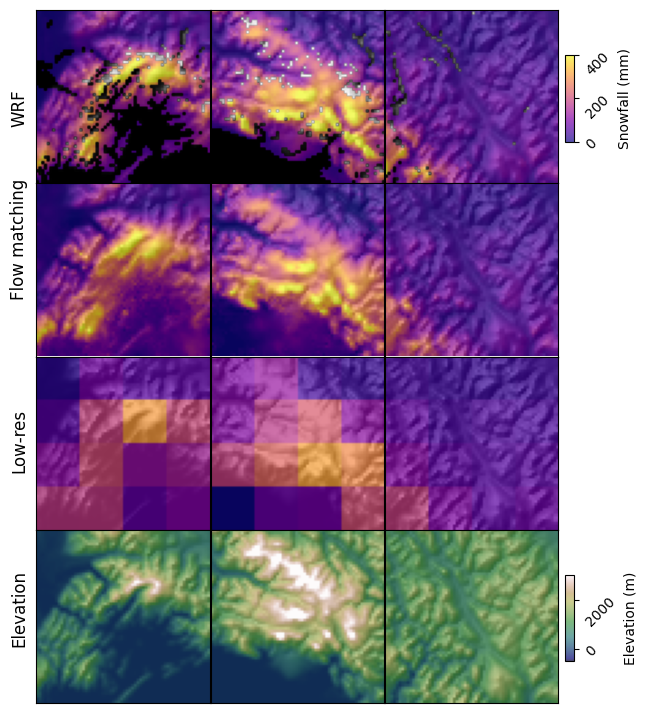
\includegraphics{figures/fig1}

\caption{Results of WRF-Flow (Flow matching) pilot study on the evaluation portion of the data.  The hi-res WRF output (a) was coarsened to produce a low-res input for WRF-Flow (c). WRF-Flow combined the elevation map and low-res input to produce a high-res output (b), which compares favorably to the original (a).
}

\label{fig1}

\end{figure}

To demonstrate its efficacy, we applied WRF-Flow to an area covering the  St. Elias and Chugach mountain ranges in southeastern Alaska.  Beginning with WRF simulation outputs at 4 km horizontal resolution, we coarsened the data to simulate 64 km resolution climate model output, and then used WRF-Flow to recreate, as best as possible, the original 4 km data.  The dataset comprises maximum 3-day snowfall accumulations from multiple atmospheric forcings: CFSR reanalysis (1981–2010) for the historical baseline and GFDL CM3 and CCSM4 climate models (2031–2060) for future projections. We partition the temporal domain into 120 time steps for training and 30+ independent time steps for evaluation.  Initial results are shown in Figure~\ref{fig1}.

\section{Ensemble Statistics and Probabilistic Predictions}

\begin{figure}
\centering

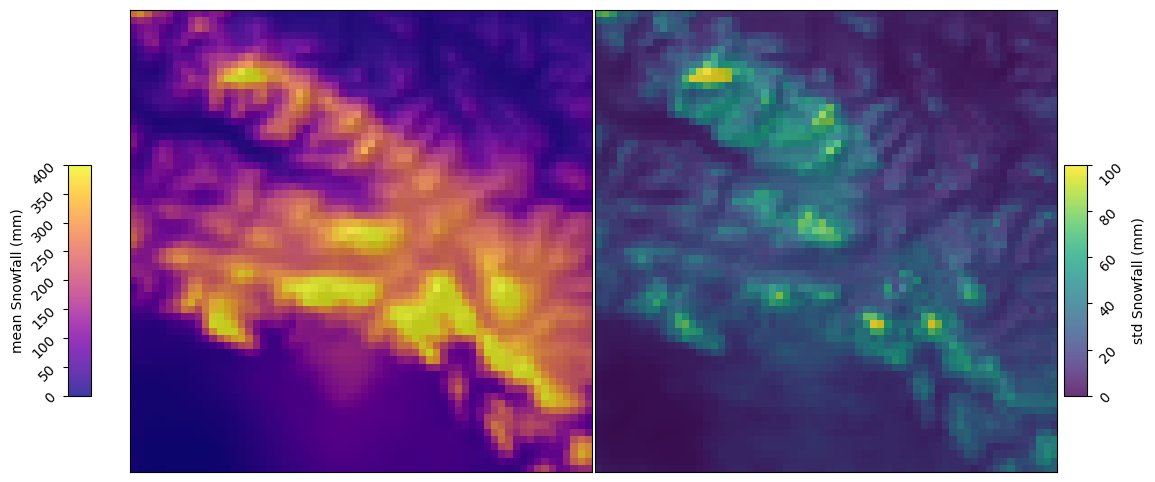
\includegraphics[width=\textwidth]{figures/fig2}

\caption{Uncertainty quantification for XXXX region.   Deviations from the mean exhibit strong spatial coherence relative to topography, and orographic effects are clearly visible.}

\label{fig2}

\end{figure}

By generating multiple independent realizations with different noise samples, we obtain an ensemble that characterizes the conditional probability distribution over the downscaling problem (Figure~\ref{fig2}). The spatial pattern of ensemble spread provides diagnostic information about which regions have high predictability (low spread) and which regions have intrinsic unpredictability relative to the coarse forcing (high spread).

A key advantage of the generative approach is the ability to draw multiple independent samples from the learned conditional distribution. By sampling different realizations of the noise and integrating the learned velocity field with the same conditioning information, we generate an ensemble of precipitation realizations consistent with both the coarse climate forcing and the high-resolution topography.



\section{Spatial Evaluation of Forecast Skill}

\begin{figure}
\centering

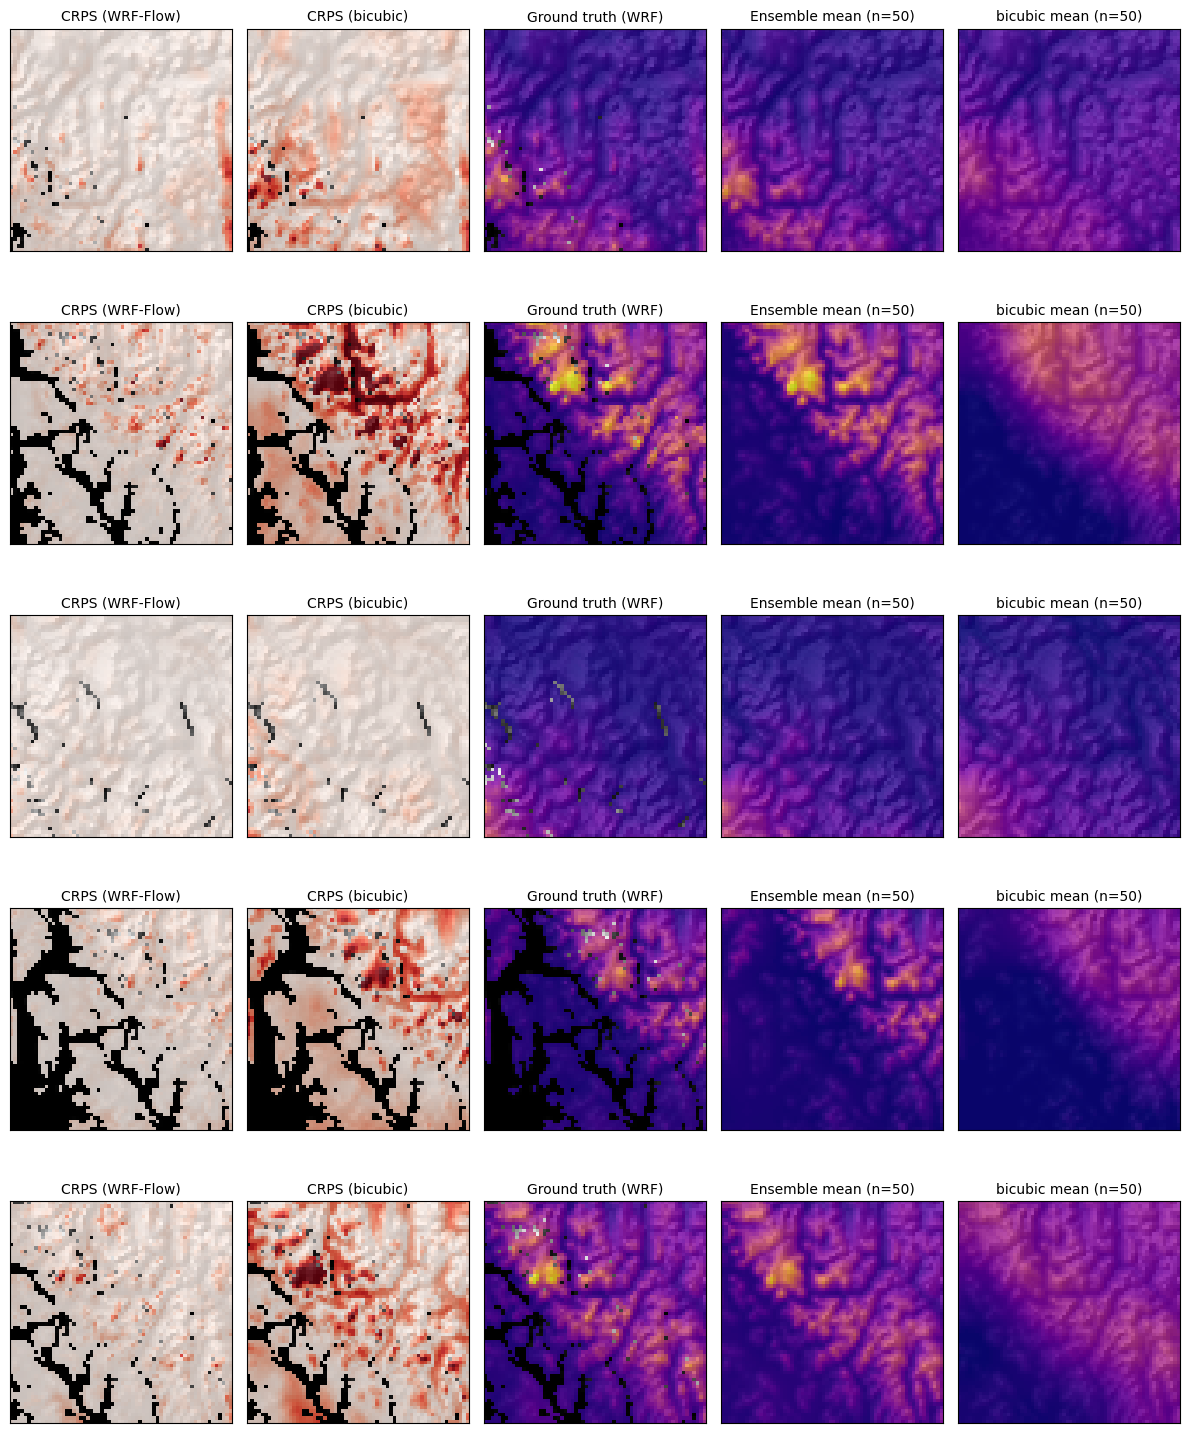
\includegraphics[width=\textwidth]{figures/fig3}

\caption{Overlays on hillshade-enhanced topography highlight the spatial coherence of predicted patterns relative to topographic forcing.}

\label{fig3}

\end{figure}

To evaluate WRF-Flow, we compare it to the baseline method, in which coarse climate data are refined via lapse rate correction.  We used Continuous Ranked Probability Score (CPRS) to evaluate each of the two methods against the original WRF output.  CPRS is a proper scoring rule that measures the calibration of probabilistic predictions, penalizing both forecast bias and overconfidence, balancing distance to the observation (reliability) against ensemble spread (resolution). Lower CRPS indicates better forecast skill.  Results (Figure~\ref{fig3}) show that WRF-Flow as a dramatic improvement to accurately place precipitation in Southeast Alaska, where orographic precipitation effects are important.


\section{Conclusion}

We have presented an application of conditional flow matching to emulating the annual maximum 3-day snowfall rates in the mountains of coastal Alaska as predicted by WRF, conditioned on high resolution topography and the low-resolution climate forcing that might be a reasonable representation of CMIP-class climate models. We call this model WRF-Flow. We find that WRF-Flow does a qualitatively good job of reproducing high-resolution simulations. The distribution over its predictions is spatially coherent, with deviations from the ensemble mean governed by topography and physically-plausible effects like rain shadowing that are evident in the training data. Under quantitative metrics like CRPS and various norms of power-spectral density, WRF-Flow improves significantly over a simple regression-based baseline. Notably WRF-Flow produces spectral consistency with WRF, albeit while exhibiting similar low-frequency biases evident in many generative models. Based on this evidence and previous work on generative modelling of ML-based downscaling of weather models that conditional flow matching has the potential to be an effective surrogate for a more complete representation of WRF predictions.

\section{Appendix: Method Details}

Conditional flow matching (CFM) is a framework for training generative models by learning velocity fields that interpolate between noise and data distributions. Unlike diffusion models, which reverse a fixed Markovian noise schedule, flow matching constructs probability paths via optimal transport, enabling more efficient training and faster sampling.

\subsection{Mathematical Framework}

Given a high-resolution precipitation field $\mathbf{x}_1 \sim p_{\mbox{\tiny data}}$ and Gaussian noise $\mathbf{x}_0 \sim \mathcal{N}(0, \mathbf{I})$, the optimal transport probability path interpolates between these distributions:

    $$\mathbf{x}_t = \sigma(t) \mathbf{x}_0 + \mu(t) \mathbf{x}_1$$
    
where $\sigma(t)$ and $\mu(t)$ are smooth monotonic functions satisfying $\sigma(0)=1, \mu(0)=0$ and $\sigma(1)=0, \mu(1)=1$. The velocity field in probability space is then:

    $$\mathbf{v}(\mathbf{x}_t, t \mid \mathbf{c}) = \dot{\mu}(t) \mathbf{x}_1 - \dot{\sigma}(t) \mathbf{x}_0$$
    
where $\mathbf{c}$ denotes the conditioning information (coarse climate and topography). To train the generative model, we parameterize the velocity field $\mathbf{v}_\theta(\mathbf{x}_t, t \mid \mathbf{c})$ via a neural network and minimize the mean squared velocity prediction error:

    $$\mathcal{L} = \mathbb{E}_{t, \mathbf{x}_1, \mathbf{x}_0, \mathbf{c}} \left\| \mathbf{v}_\theta(\mathbf{x}_t, t \mid \mathbf{c}) - \mathbf{v}(\mathbf{x}_t, t \mid \mathbf{c}) \right\|_2^2$$
    
masked to exclude pixels with missing precipitation data. This objective directly minimizes the distance between predicted and target velocity fields, providing a more stable optimization target than score matching used in diffusion models.






% --------------------------------------
\subsection{Architecture: Conditional U-Net with Self-Attention}
    
We employ a U-Net architecture with hierarchical feature extraction and self-attention mechanisms to approximate the conditional velocity field $\mathbf{v}_\theta$. The network is designed to balance computational efficiency with expressiveness sufficient to capture multi-scale precipitation patterns.
    
The architecture operates on 4-channel input concatenating (1) the partially denoised precipitation $\mathbf{x}_t$, (2) the high-resolution topography $z$, (3) the coarse-resolution climate model output $\bar{\mathbf{x}}_c$, and (4) a binary validity mask indicating missing data regions. The output is a single-channel velocity field prediction.

The forward pass follows the standard U-Net pattern: an initial convolution expands the spatial resolution to the base channel dimension, a sequence of downsampling blocks progressively reduce spatial resolution while increasing feature depth, a bottleneck layer applies processing at the coarsest resolution, and symmetric upsampling blocks with skip connections restore spatial resolution while progressively decreasing channels.

\begin{itemize}

\item \textbf{Time conditioning:} Sinusoidal embeddings of the time variable $t$ are computed via:

\begin{equation}
\mathbf{e}_t^{(j)} =
  \begin{cases}
    \sin(10000^{-2j/d} \cdot t)    & \mbox{if } j \mbox{ is even} \\
    \cos(10000^{-2(j-1)/d} \cdot t) & \mbox{if } j \mbox{ is odd}
  \end{cases}
\end{equation}

These embeddings are projected via an MLP and added to feature maps at each ResBlock, allowing the network to modulate feature processing as a function of the denoising progress.


\item \textbf{Multi-scale Attention:} Self-attention layers are applied at 16×16 resolution (intermediate depth of the U-Net hierarchy), enabling the network to capture long-range spatial dependencies in precipitation patterns. This resolution balances the computational cost of attention operations with the need to model large-scale orographic forcing.

\item \textbf{Normalization and Regularization:} Group normalization (with 32 groups) stabilizes training across variable batch sizes and provides robustness to initialization. Dropout is applied during training to regularize the network and reduce overfitting, particularly important given the modest dataset size.

\end{itemize}

% --------------------------------------


\subsection{Training Procedure}
    
    We train the velocity network via gradient descent on the velocity prediction loss (Equation 3 above) over mini-batches of (coarse, fine, topography) triplets sampled from the training set. 

\begin{itemize}
    
\item \textbf{Optimization:} Adam optimizer with learning rate $2 \times 10^{-4}$, $\beta_1 = 0.9$, $\beta_2 = 0.999$.
    

\item \textbf{Data Sampling:} Mini-batches of size 24 are randomly sampled from the 120 training time steps, with random spatial tiling applied at each iteration. To counteract the rapid initial signal decay early in the denoising trajectory, the time variable $t$ is sampled with bias toward the latter portion of the [0, 1] interval, increasing the relative importance of the refined precipitation features that emerge as $t \to 1$.
    
\item \textbf{Training Duration:} 10,000 optimization steps, corresponding to approximately 2.5 epochs through the training dataset given the random tiling strategy.
    

\item \textbf{Masked Loss:} The loss is computed only over pixels with valid (non-missing) precipitation observations, preventing the network from learning to predict velocity in regions where ground truth is unavailable. Checkpoints are saved every 100 steps to enable recovery from training interruption and model selection based on validation loss.
    
\end{itemize}

% --------------------------------------

\subsection{Generation via ODE Integration}
    
Given a trained velocity network $\mathbf{v}_\theta$, we generate new samples by integrating an ordinary differential equation in probability space. Sampling from noise $\mathbf{x}_0(t=0) \sim \mathcal{N}(0, \mathbf{I})$ and integrating the learned velocity field:

    $$\frac{d\mathbf{x}}{dt} = \mathbf{v}_\theta(\mathbf{x}(t), t \mid \mathbf{c})$$

\noindent from $t=0$ to $t=1$ with fixed conditioning $\mathbf{c}$ (coarse precipitation and topography), we obtain a sample $\mathbf{x}_1 = \mathbf{x}(t=1)$ from the learned conditional distribution. The ODE is integrated using an adaptive-step Runge-Kutta solver (DOPRI5) with relative and absolute tolerances of $10^{-5}$, requiring approximately 10 function evaluations per sample.


% --------------------------------------






\end{document}
